%--------------------------------------------------------------------------------
%
% Text příspěvku do sborníku EEICT
%
% Vytvořil:  Martin Drahanský
% Datum:     26.02.2007
% E-mail:    drahan@fit.vutbr.cz
%
%--------------------------------------------------------------------------------
%
% Přeložení: pdflatex prispevek.tex
%
% Optimální způsob použití = přepište jen vlastní text
%
\documentclass{eeict}
\inputencoding{utf8}
\usepackage[bf]{caption2}
%--------------------------------------------------------------------------------

%%% MOJE
\graphicspath{{obr/}{obr/plots/}{spice/}}
\DeclareGraphicsExtensions{.ps, .eps}
%\usepackage[slovak]{babel}
%\usepackage[utf8]{inputenc} 
\usepackage{amsmath}
\usepackage{listings}

\newcommand{\dif}{\, \mathrm{d}}	% diferencia (na derivacie)
\newcommand{\difp}{\partial}		% parc. diferencia 
\newcommand{\dxdt}[2]{\frac{\mathrm{d} #1}{\mathrm{d} #2}}
\newcommand{\dxdtp}[2]{\frac{\partial #1}{\partial #2}}
\newcommand{\un}[1]{\, \mathrm{#1}}	% jednotky velicin, v math mode
\newcommand{\E}[1]{\cdot 10^{#1}}
\newcommand{\degree}{^\circ}
\newcommand{\diameter}{\emptyset}
\newcommand{\cpx}{\widehat}		% komplexne fazory
\newcommand{\Ohm}{\Omega}

\lstnewenvironment{mycode1}
{
	%\begin{lstlisting}[language=Python, morekeywords=inner, morekeywords=solve]
	\lstset{
		%language=Python,
		%morekeywords=Expression
		language=Python,
		%basicstyle=\ttfamily\footnotesize,
		basicstyle=\ttfamily\footnotesize,
		keywordstyle = \bfseries,
		breaklines=true,
		showstringspaces=false,
		%numbers = left,
		frame=single,
		%otherkeywords={Test, Trial, Function, Expression, solve, dot, inner, grad}
		morekeywords={Mesh, RectangleMesh, IntervalMesh, Point, FunctionSpace, TestFunction, TrialFunction, Function, Expression, solve, dot, inner, grad}
	}
}
{
	%\end{lstlisting}
}

\newcommand{\myfig}[3]
{
    \begin{figure}[!ht]
    %\begin{figure}[ht]
    %\begin{figure}[htpb]
	\centering
	\includegraphics{#1}
	\caption{#2}
	%\label{fig:#3}
	#3
    \end{figure}
}
\newcommand{\myfigsc}[3]
{
    \begin{figure}[!ht]
	\centering
	\includegraphics[width=3.5in]{#1}
	\caption{#2}
	%\label{fig:#3}
	#3
    \end{figure}
}
%--------------------------------------------------------------------------------


\title{TITLE OF THE PAPER - IN ENGLISH}
\author{Ján Mikláš}
\programme{Doctoral Degree Programme (1), FEEC BUT}
\emails{jan.miklas@vutbr.cz}

\supervisor{Petr Procházka}
\emailv{prochazkap@feec.vutbr.cz}

\abstract{The abstract is placed here. It shoud be approximately 50-100 words long.
The purpose of the abstract is to summarize the important ideas of the paper. It
must be written in English. Please ask your supervisor to check the abstract. 
Below the abstract there are keywords there, also written in English.}
\keywords{EEICT, template, guide}

\begin{document}
% -- Hlavička práce --

\maketitle

%-------------------------------------------------------------------------------
\selectlanguage{czech}
%\selectlanguage{english}
\section*{Abstrakt}
<+blablabla+>
Modelom budú (sú) demonštrované základné javy vedenia prúdu cez PN prechod ako sú: driftový prúd, difúzny prúd, vytvorenie vyprázdnenej oblasti pri závernom pólovaní, injekcia minorítných nosičov do opačne dotovaných oblastí pri priepustnom pólovaní, volt-ampérová charateristika a jej zodpovedajúce priestorové rozloženie eletrónov a dier.

\section{Úvod}


\section{Rovnice polovodičov}
Význam použitých symbolov:\\
\begin{tabular}{l l l}
	\hline
	$\varepsilon$ & permitiivta prostredia (kremíku)\\
	$\psi$ & elektrický potenciál \\
	$\mathbf{E}$ & intenzita elektrického poľa\\
	$q$ & náboj elektrónu\\
	$p, n$ & koncentrácie dier a elektrónov\\
	$N_D, N_A$ & koncentrácie donorov a akceptorov\footnotemark\\
	$\mathbf{J_n}, \mathbf{J_p}$ & prúdy elektrónov a dier jednotkou plochy\\
	$\mu_n, \mu_p$ & pohyblivosti nosičov\\
	$D_n, D_p$ & difúzne konštanty (Fickov zákon)\\
	$U_n, U_p$ & miera generácie a rekombinácie elektrónov a dier\\
	\hline \\
\end{tabular}
\footnotetext{Pre jednoduchosť stačí uvažovať prípad, kde všetky prímesové atómy sú zionizované.}

Poissonova rovnica\footnote{Jedna z Maxwellovych rovníc v diferenciálnom tvare \mbox{$\nabla \cdot \mathbf{D} = \rho$}, kde \mbox{$\mathbf{D} = \varepsilon E \implies \nabla \cdot (\varepsilon \nabla \psi) = - \rho$}}:
\begin{equation}
	\nabla \cdot (\varepsilon \nabla \psi) = -q (p -n + N_D - N_A)
	\label{eq:poisson}
\end{equation}

Prúdy:
\begin{equation}
	\mathbf{J_n} = \overbrace{q n \mu_n \mathbf{E}}^\text{drift} + \overbrace{q D_n \nabla n}^\text{difúzia}
	\label{eq:Jn}
\end{equation}
\begin{equation}
	\mathbf{J_p} = q p \mu_p \mathbf{E} - q D_p \nabla p
	\label{eq:Jp}
\end{equation}

Rovnice kontinuity (zachovanie resp. časová spojitosť náboja):
\begin{equation}
	\dxdtp{n}{t} = \nabla \cdot \mathbf{J_n} + U_n
	\label{eq:continuity_n}
\end{equation}
\begin{equation}
	\dxdtp{p}{t} = -\nabla \cdot \mathbf{J_p} - U_p
	\label{eq:continuity_p}
\end{equation}

Je dobré pripomenúť vzťah $\mathbf{E} = - \nabla \psi$. Prvý sčítanec na pravej strane rovníc (\ref{eq:Jn}) a (\ref{eq:Jp}) predstavuje driftový prúd (daný pohyblivosťou nábojov a intenzitou elektrického poľa), druhý sčítanec predstavuje difúzny prúd podľa prvého Fickovho zákona, teda úmerný spádu koncentrácie nábojov a difúznej konštante.

Rovnice (\ref{eq:poisson}) až (\ref{eq:continuity_p}) tvoria sústavu vzájomne previazaných nelineárnych rovníc s 5 neznámzmi ($\psi, \mathbf{J_n}, \mathbf{J_p}, n, p$). Dosadením (\ref{eq:Jn}) do (\ref{eq:continuity_n}) a (\ref{eq:Jp}) do (\ref{eq:continuity_p}) je možné riešiť 3 rovnice s neznýmymi ($\psi, n, p$). Tento postup bude využitý v stati \ref{ch:implementacia__matematicke_upravy}.


\section{MKP, FEniCS a stratégia riešenia}
K numerickému riešeniu rovníc polovodičov použijeme diskretizáciu metódou konečných prvkov (MKP) s využitím programových nástrojov akademicko - vedeckej výpočtovej platformy FEniCS \cite{fenicsproject}.

<+Variacna forma+>
<+Mixed formy vs decoupling+>
<+Casova diskretizacia+>

\section{Implementácia}<++>
\subsection{Matematické úpravy}\label{ch:implementacia__matematicke_upravy}<++>
Dosadením (\ref{eq:Jn}) do (\ref{eq:continuity_n}) a (\ref{eq:Jp}) do (\ref{eq:continuity_p}) a vyžitím vzťahu $\mathbf{E} = - \nabla \psi$ dostávame nasledovnú sústavu rovníc s 3 neznýmymi ($\psi, n, p$) - tj. Poissonovu rovnicu a rovnice kontinuity elektónov a dier:
\begin{equation}
	\nabla \cdot (\varepsilon \nabla \psi) = -q (p -n + N_D - N_A)
	\label{eq:poisson2}
\end{equation}
\begin{equation}
	\dxdtp{n}{t} = \nabla \cdot (-n \mu_n \nabla \psi + D_n \nabla n) + U_n
	\label{eq:continuity_n2}
\end{equation}
\begin{equation}
	\dxdtp{n}{t} = \nabla \cdot (-p \mu_p \nabla \psi - D_p \nabla p) + U_p
	\label{eq:continuity_p2}
\end{equation}
<+stále sú vzájomne previazané+> To je dosť závažná nepríjemnosť.

<+Poissonova rovnica - varacna forma atd\footnote{$\dif{x}$ predstavuje vektor takého rozmeru, ako je rozmer priestorových súradníc riešenej úlohy}+>

Časová diskretizácia rovnice (\ref{eq:continuity_n2}):
\begin{equation}
	\frac{n_{i} - n_{i-1}}{dt} = \nabla (-\mu_n n_{i-1} \nabla \psi_i) + \nabla \cdot \left( D_n \nabla n_i \right) + U_n
	\label{eq:continuity_n_diskr}
\end{equation}

\begin{equation}
	n_i - \nabla \cdot (dt D_n \nabla n_i) = n_{i-1} - \nabla (dt \mu_n n_{i-1} \nabla \psi_i) + dt U_n			
	\label{eq:continuity_n_diskr_ni}
\end{equation}
Z toho bilineárna a lineárna forma pre MKP $a(n, v) = L(v)$ (neznámu $n_i$ budeme ďalej označovať jednoducho $n$) získaná vynásobením oboch strán (\ref{eq:continuity_n_diskr_ni}) testovacou funkciou $v$ a následným integrovaním podľa $\dif{x}$:
\begin{equation}
	\begin{array}{l l}
		\int_{\Omega} n v \dif x + \int_{\Omega} dt D_n \nabla n \nabla v \dif x
		=\\
		= \int_{\Omega} n_{i-1} v \dif x - \int_{\Omega}dt \mu_n n_{i-1} \nabla \psi_i \nabla v \dif x + \int_{\Omega} dt U_n v \dif x
	\end{array}
	\label{eq:continuity_n_a_L}
\end{equation}

(\ref{eq:continuity_p2})
 
\subsection{Okrajové podmienky}<++>
\subsection{Scaling}
Pokiaľ majú výsledky - predovšetkým elektrických veličín ako potenciál či prúdové hustoty - kvantitatívne zodpovedať realistickým hodnotám, je nutné aplikovať realistické hodnoty materiálových i rozmerových konštánt. Tým však vzniknú obrovské rozdiely v rádoch jednotlivých veličín, čo má za následok jednak zbytočne vysokú výpočtovú cenu (resp. čas výpočtov), jednak možnú stratu numerickej riešiteľnosti. Preto sa rovnice násobia ešte pred výpočtom škálovacími konštantami \cite{selberherr} \cite{de_mari} a následne sa spätne \uv{zrozmerňujú} až výsledky.

Účelom tohto článku je odvodenie a zostavenie výpočtového modelu s následným kvalitatívnym overením jeho funkčnosti. Pre jednoduchosť bude preto tento model bezrozmerný, tj. konštanty budú jednotkové.
%\subsection{Výpočtové prevednie (program)}
\subsection{Výpočtové prevednie (Python)}


\begin{mycode1}
# Mesh and function space
nx = 100
ny = 1
mesh = RectangleMesh(Point(0.0, 0.0), Point(x_length, y_length) , nx, ny, 'crossed')
V = FunctionSpace(mesh, "CG", 1)
Vn=V
Vp=V
\end{mycode1}

\begin{mycode1}
####################
## Poisson
####################
rho = Expression("q * (p - n + Nd - Na)", q=q, p=p0, n=n0, Nd=Nd, Na=Na, degree=1)
Psi = TrialFunction(V)
v_psi = TestFunction(V)
a = -inner(grad(Psi), grad(v_psi)) * dx
L = -rho/eps_Si*v_psi*dx

Psi_result = Function(V)
#solve(a==L, Psi_result, [bc_psi1, bc_psi2])
\end{mycode1}

\begin{mycode1}
####################
## n, p Continuity
####################
n_i1 = Function(Vn)
n_i1.assign(n0)
n = TrialFunction(Vn)
vn = TestFunction(Vn)
#an = n*vn*dx + dt*Dn*inner(grad(n), grad(vn))*dx
an = n*vn*dx + dt*D_n*inner(grad(n), grad(vn))*dx
Ln = n_i1*vn*dx + dt*mob_n*n_i1*inner(grad(Psi_result), grad(vn))*dx

n_result = Function(Vn)
#solve(an==Ln, n_result, [bc_n1, bc_n2])

p_i1 = Function(Vp)
p_i1.assign(p0)
p = TrialFunction(Vp)
vp = TestFunction(Vp)
ap = p*vp*dx + dt*D_p*inner(grad(p), grad(vp))*dx
Lp = p_i1*vp*dx - dt*mob_p*p_i1*inner(grad(Psi_result), grad(vp))*dx

p_result = Function(Vp)
#solve(ap==Lp, p_result, [bc_p1, bc_p2])
\end{mycode1}

\begin{mycode1}
Psi_result = Function(V)
n_result = Function(Vn)
p_result = Function(Vp)
#solve(a==L, Psi_result, [bc_psi1, bc_psi2])
#solve(an==Ln, n_result, [bc_n1, bc_n2])
#solve(ap==Lp, p_result, [bc_p1, bc_p2])
\end{mycode1}

\section{Príklad riešenia - PN prechod; rovnovážny stav, napäťové okrajové podmienky}<++>
\myfigsc{tmp1}{}{}
\myfigsc{tmp2}{}{}
\myfigsc{tmp3}{}{}
\myfigsc{tmp4}{}{}
\subsection{Interpretácia výsledkov}<++>
\subsubsection{Koncentrácie voľných nosičov}<++>
\subsubsection{Driftový a difúzny prúd}<++>
%\myfig{obr.jpg}{aa}{\label{fig:aa}}
%\myfig{iter-1-J.eps}{}{}
%\myfigscaled{iter-1-J.eps}{width=0.8\columnwidth}{Aaaa.}{\label{fig:aaaa}}


%\begin{thebibliography}{9}
%\bibitem{lit:shockley}<++>
%\bibitem{lit:pierret}<++>
%\bibitem{lit:gummel}<++>
%\bibitem{lit:fenicsbook}<++>
%\end{thebibliography}

% bibtex:
\nocite{fenicsbook}
\nocite{brenner_scott}
%\bibliographystyle{plain}
\bibliographystyle{unsrt}
\bibliography{../lit}

%\input{./kapitoly/prilohy}
\appendix
\section{Zdrojový kód (Python)}<++>

%\chapter{Obvodové schémy, zoznam súčiastok a DPS} \label{ch:priloha_schemy}

\newpage
\section{Budič výkonových tranzistorov} \label{sec:append_budic}

\hspace{-1.8cm}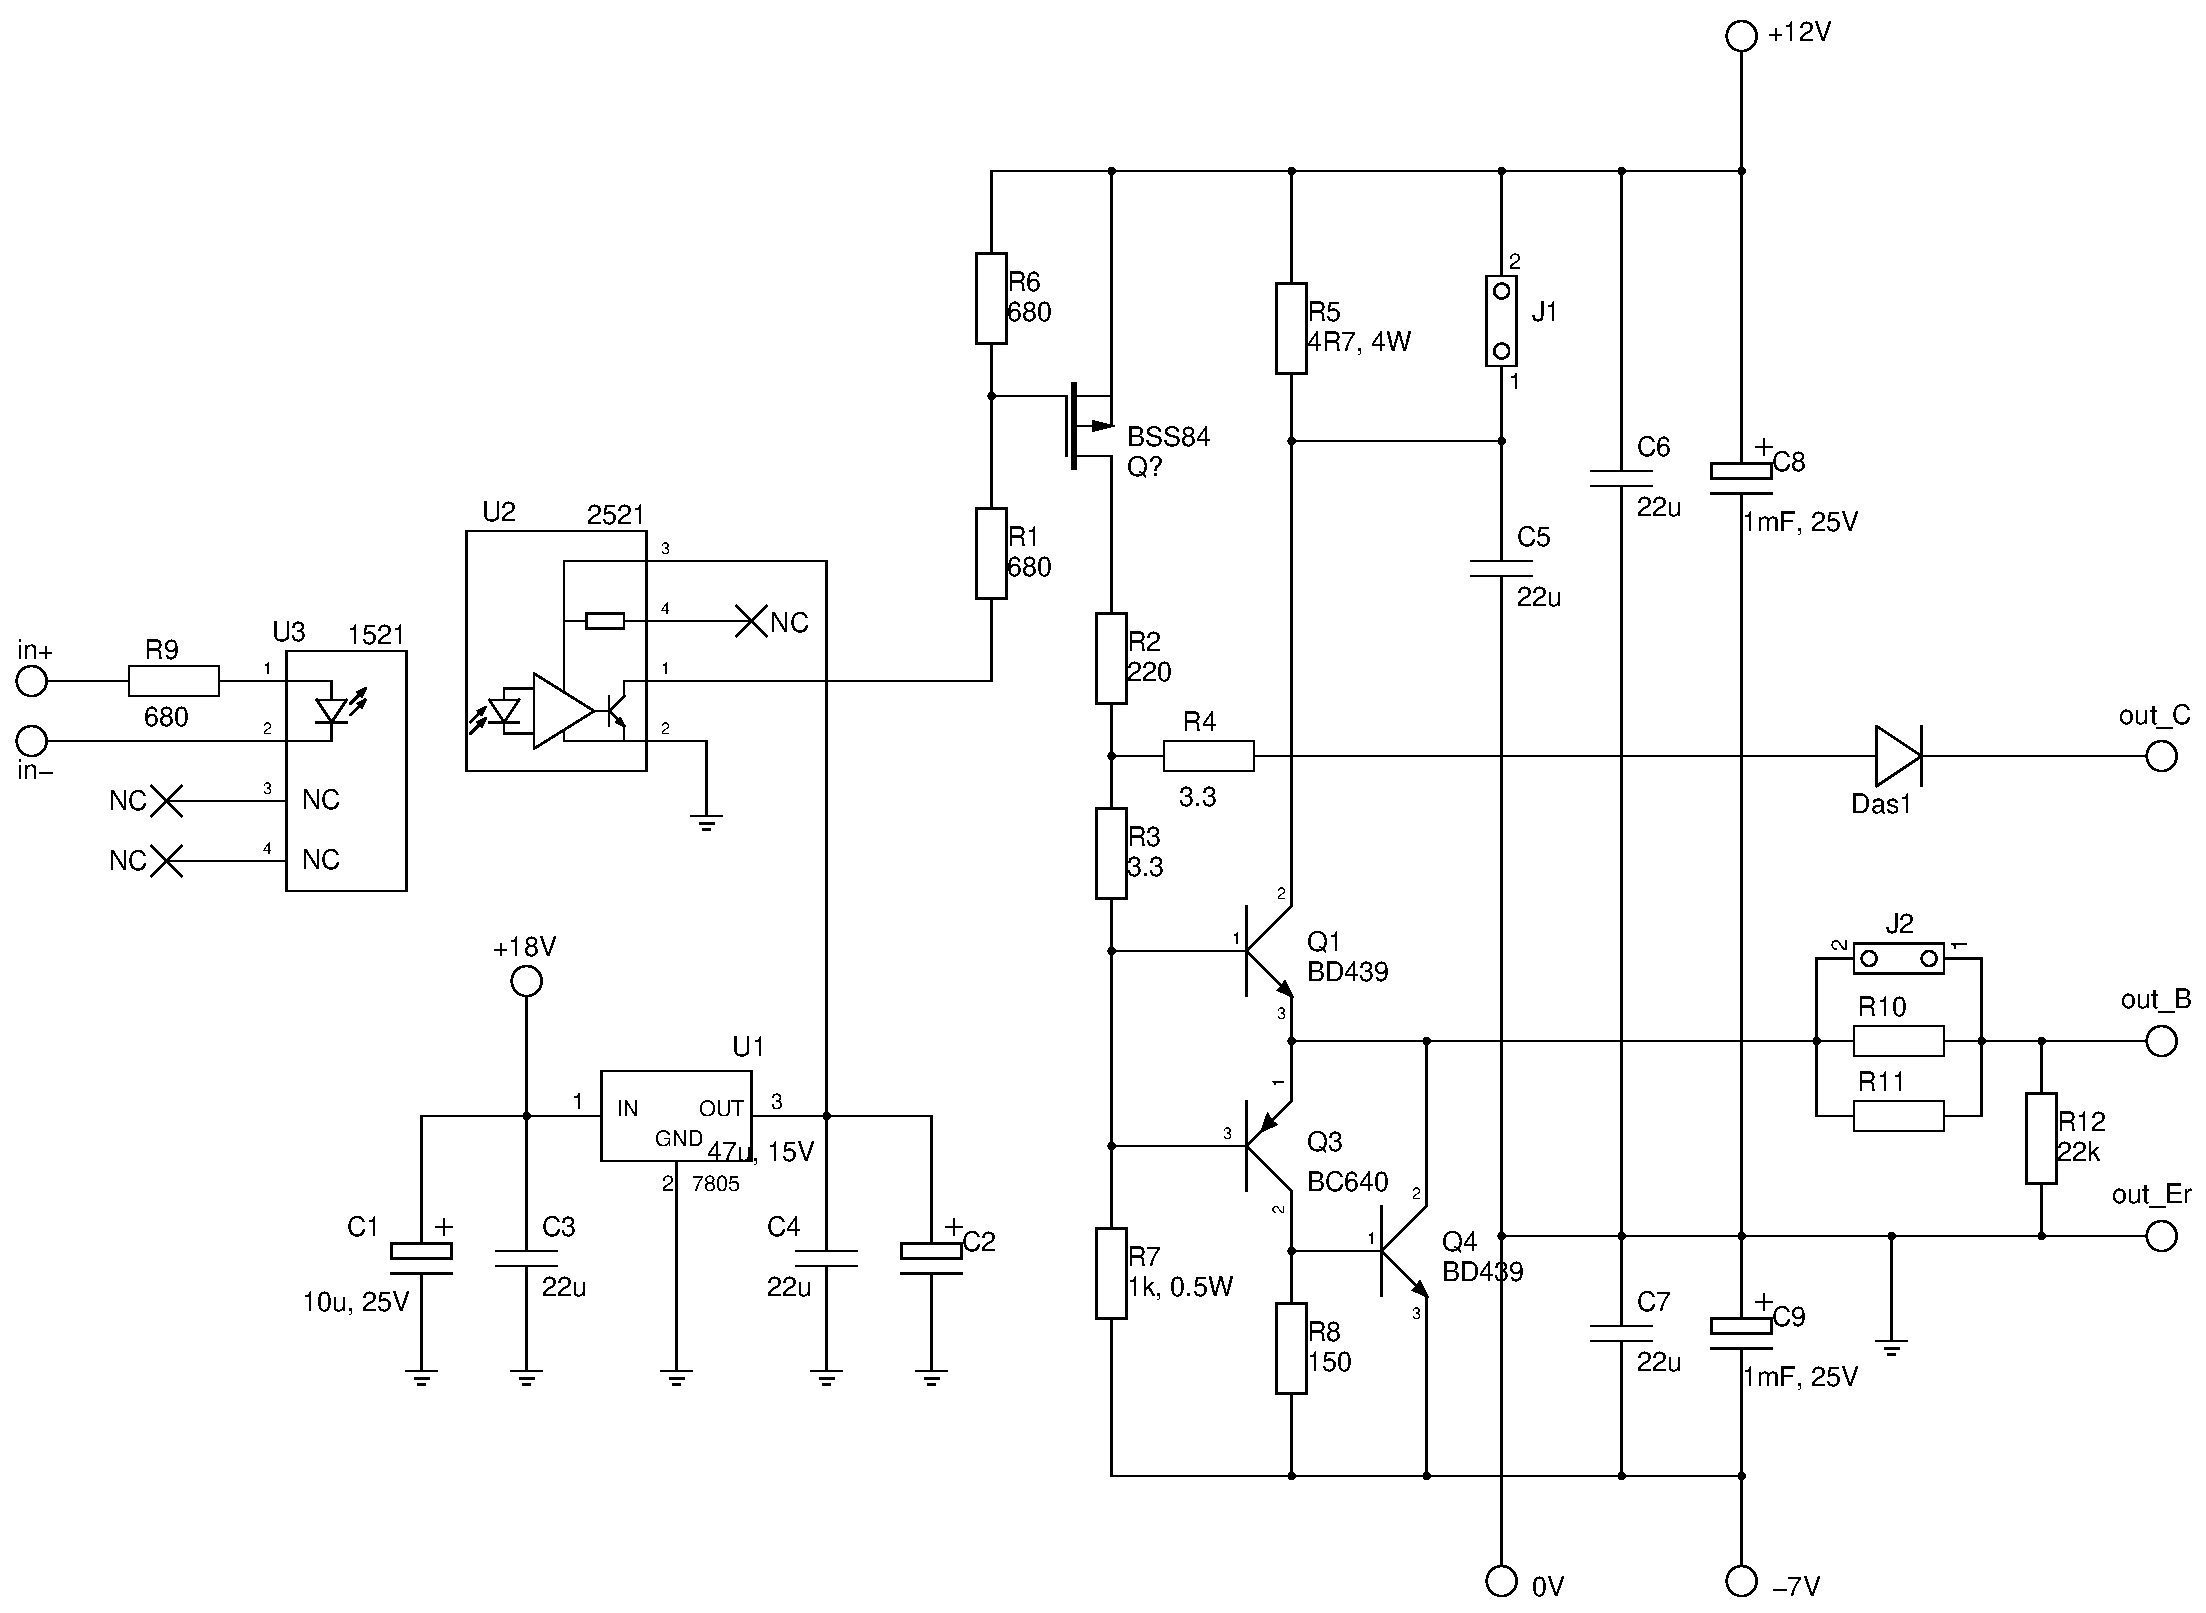
\includegraphics[width=1.2\textwidth]{schema_budic2}


\subsection{DPS}
DPS a rozmiestnenie súčiastok(1:1). Zľava: top assembly, bottom, bottom assembly:\vspace{0pt}

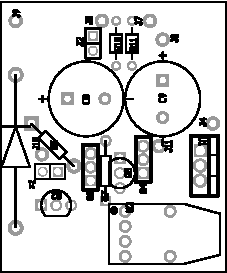
\includegraphics{pcb_budic_top_ass}
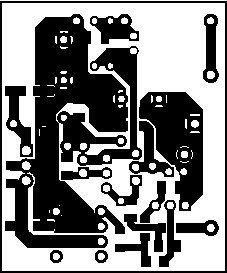
\includegraphics{pcb_budic_bot}
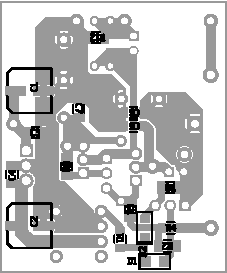
\includegraphics{pcb_budic_bot_ass}

\newpage
\subsection{Zoznam súčiastok}
\small
\begin{verbatim}

refdes   device                    footprint                     value    

C1       POLARIZED_CAPACITOR       NICHICON_WT_CAP_6p3_7p7       10u/25V
C2       POLARIZED_CAPACITOR       NICHICON_WT_CAP_6p3_7p7       47u/15V
C3       CAPACITOR                 1206.fp                       22u
C4       CAPACITOR                 1206.fp                       22u
C5       CAPACITOR                 1206.fp                       22u
C6       CAPACITOR                 1206.fp                       22u
C7       CAPACITOR                 1206.fp                       22u
C8       POLARIZED_CAPACITOR       RCY250P                       1mF/25V
C9       POLARIZED_CAPACITOR       RCY250P                       1mF/25V
D1       DIODE                     minimelf                      1N4148
D2       DIODE                     minimelf                      1N4148
Das1     DIODE                     DIODE_LAY 800.fp              [1000V]
J1       JUMPER                    JUMPER2.fp                             
J2       JUMPER                    JUMPER2.fp                             
Q1       NPN_TRANSISTOR            TO126W.fp                     BD439    
Q2       PNP_TRANSISTOR            TO92.fp                       BC640    
Q3       PNP_TRANSISTOR            TO92.fp                       BC640    
Q4       NPN_TRANSISTOR            TO126W.fp                     BD439    
R1       RESISTOR                  1206.fp                       3k3      
R2       RESISTOR                  1206.fp                       220      
R3       RESISTOR                  1206.fp                       33       
R4       RESISTOR                  1206.fp                       33       
R5       RESISTOR                  ACY400                        "4R7/4W"          
R6       RESISTOR                  1206.fp                       1k       
R7       RESISTOR                  ACY300                        "2k2/0.5W"        
R8       RESISTOR                  1206.fp                       150
R9       RESISTOR                                                680
R10      RESISTOR                  0.125W_Carbon_Resistor                 
R11      RESISTOR                  0.125W_Carbon_Resistor                 
R12      RESISTOR                  1206.fp                       22k      
U1       7805                      TO220W.fp                              
U2       fiber_optic_receiver                                    2521     
U3       fiber_optic_transmitter                                 1521     
\end{verbatim}
\normalsize
\newpage
\section{Napájací obvod budiča} \label{sec:append_nap}
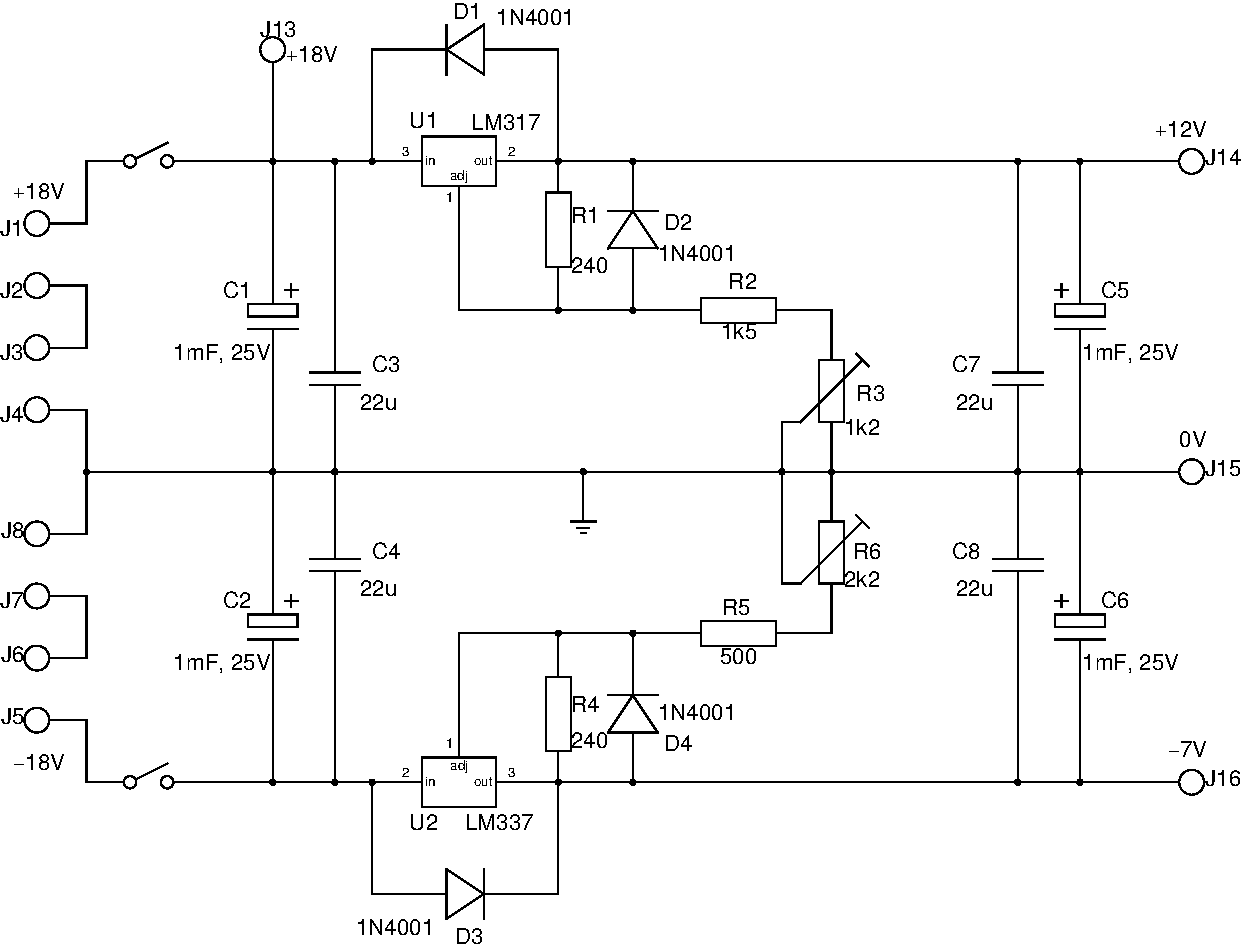
\includegraphics[width=.8\textwidth]{schema_nap}

\subsection{DPS}
DPS a rozmiestnenie súčiastok. Zľava: top assembly, bottom, bottom assembly:\vspace{5pt}

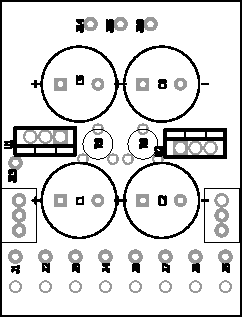
\includegraphics{pcb_nap_top_ass}
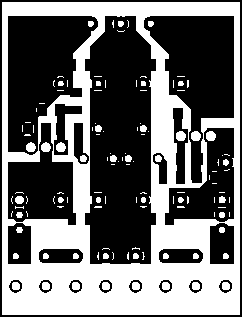
\includegraphics{pcb_nap_bot}
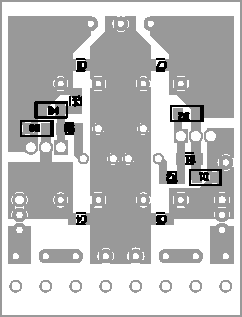
\includegraphics{pcb_nap_bot_ass}

\newpage
\subsection{Zoznam súčiastok}
\small
\hspace{2cm}
\begin{verbatim}
refdes   device                         footprint            value    

C1       POLARIZED_CAPACITOR            RCY250P              1mF/25V
C2       POLARIZED_CAPACITOR            RCY250P              1mF/25V
C3       CAPACITOR                      1206                 22u      
C4       CAPACITOR                      1206                 22u      
C5       POLARIZED_CAPACITOR            RCY250P              1mF/25V
C6       POLARIZED_CAPACITOR            RCY250P              1mF/25V
C7       CAPACITOR                      1206                 22u      
C8       CAPACITOR                      1206                 22u      
D1       DIODE                          melf                 1N4007   
D2       DIODE                          melf                 1N4007   
D3       DIODE                          melf                 1N4007   
D4       DIODE                          melf                 1N4007   
R1       RESISTOR                       1206                 240      
R2       RESISTOR                       1206                 1k5      
R3       VARIABLE_RESISTOR              trimmer_lezaty_5mm   1k2      
R4       RESISTOR                       1206                 240      
R5       RESISTOR                       1206                 500      
R6       VARIABLE_RESISTOR              trimmer_lezaty_5mm   2k2      
U1       adjustable_voltage_regulator   TO220W               LM317    
U2       adjustable_voltage_regulator   TO220W               LM337    
\end{verbatim}
\normalsize




\newpage
\section{Generátor impulzov} \label{sec:append_gen}

\subsection{Schéma zapojenia}
\hspace{-1.0cm}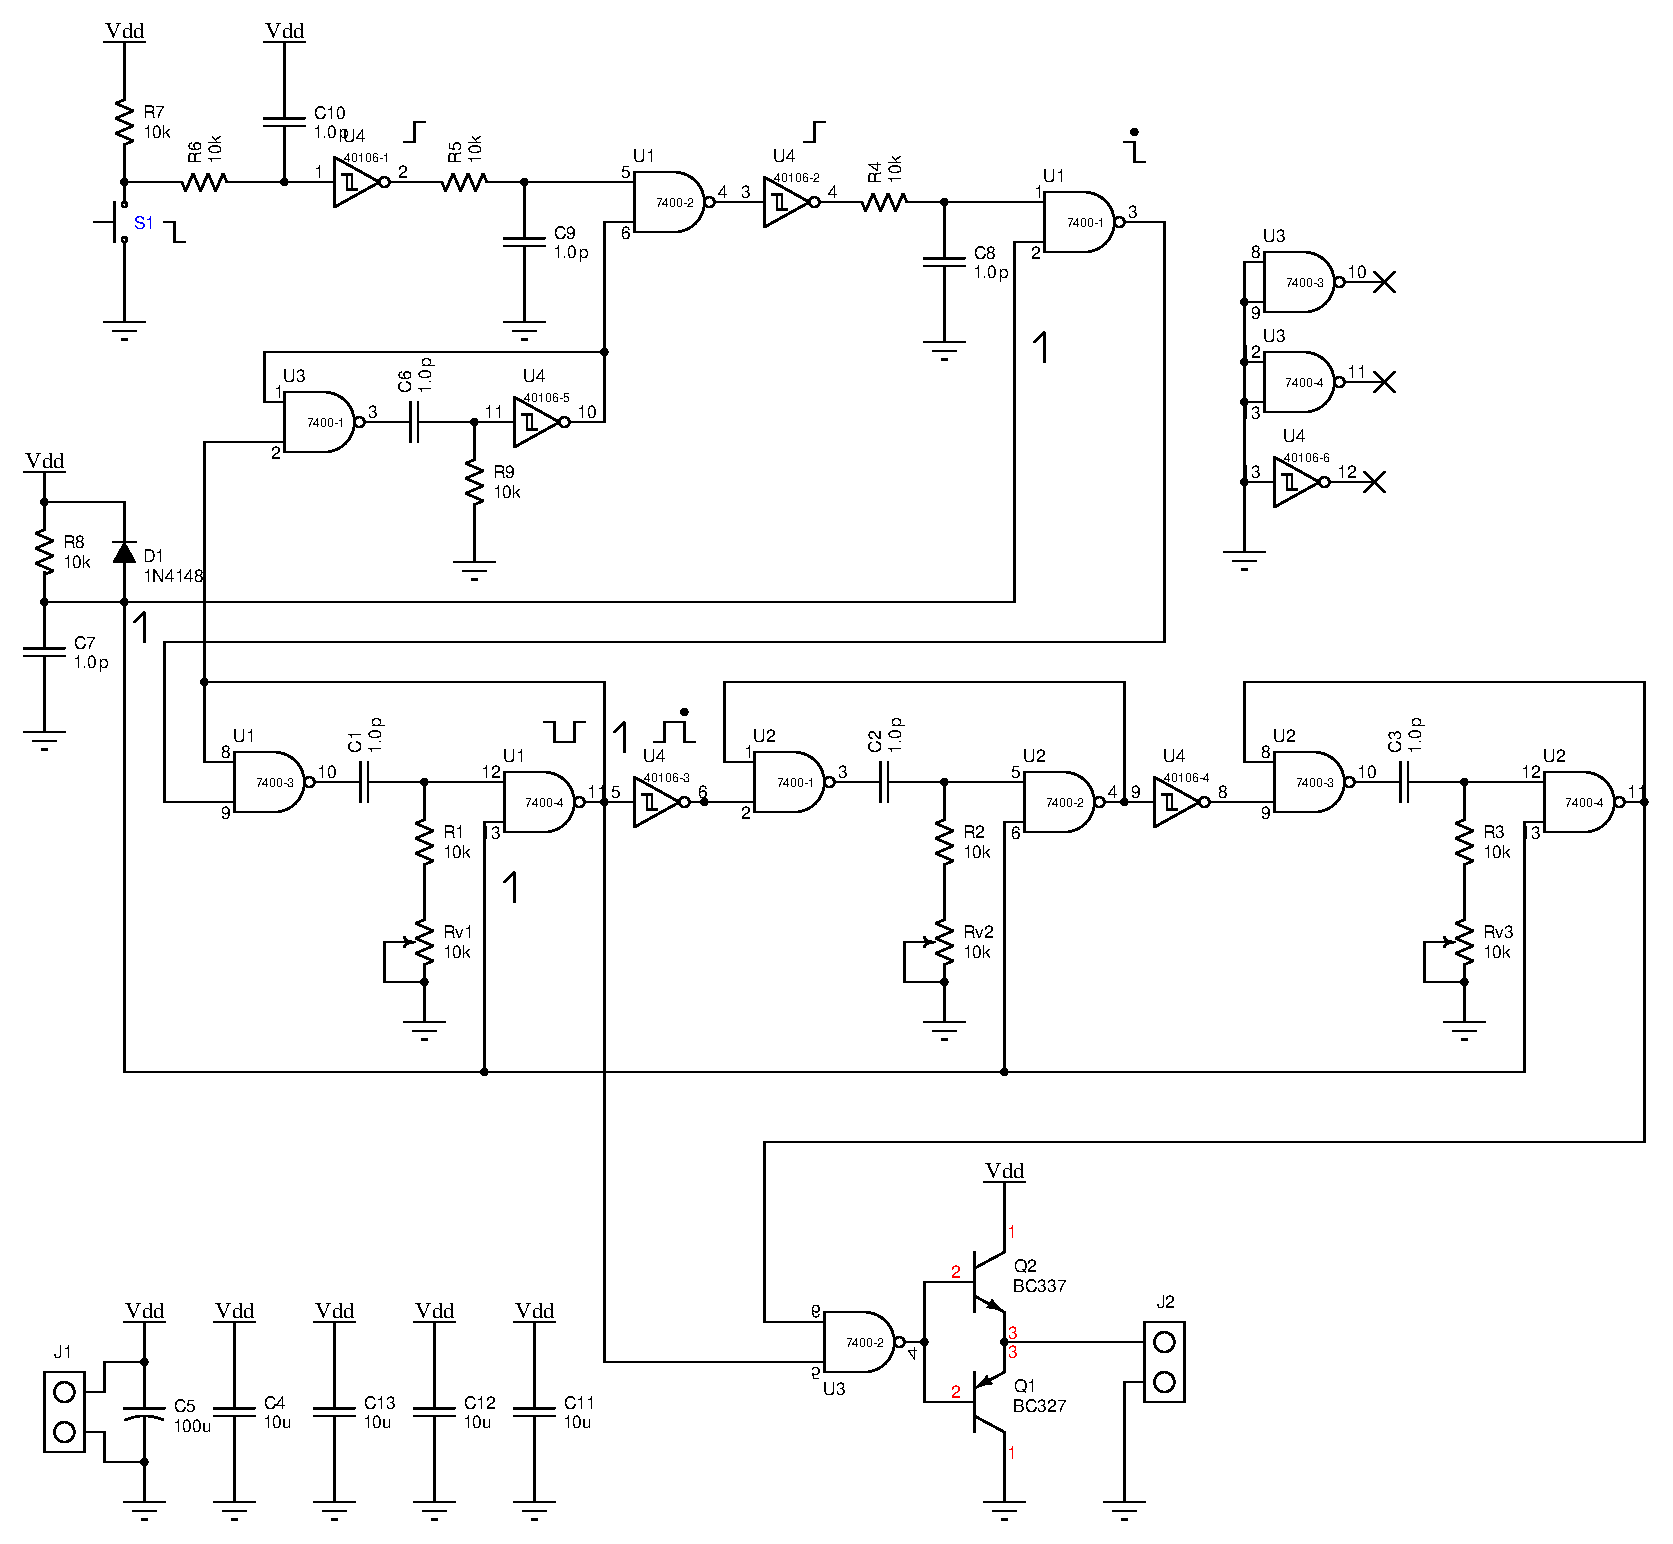
\includegraphics[width=1.25\textwidth]{schema_gen}

\newpage
\subsection{DPS}
DPS a rozmiestnenie súčiastok (1:1). Zľava: top assembly, bottom:\vspace{5pt}

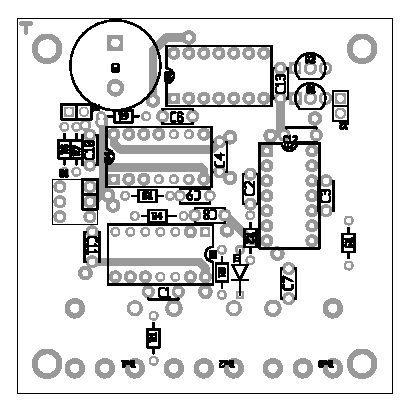
\includegraphics{pcb_gen_top_ass}

\includegraphics{pcb_gen_bot}

%\newpage
%\subsection{Zoznam súčiastok}
%\small
%\hspace{2cm}
%\begin{verbatim}
%\end{verbatim}
\normalsize



\newpage
\section{Medziobvod} \label{sec:append_medziobvod}

\subsection{Schéma zapojenia}
\vspace{10pt}
\hspace{-1.0cm}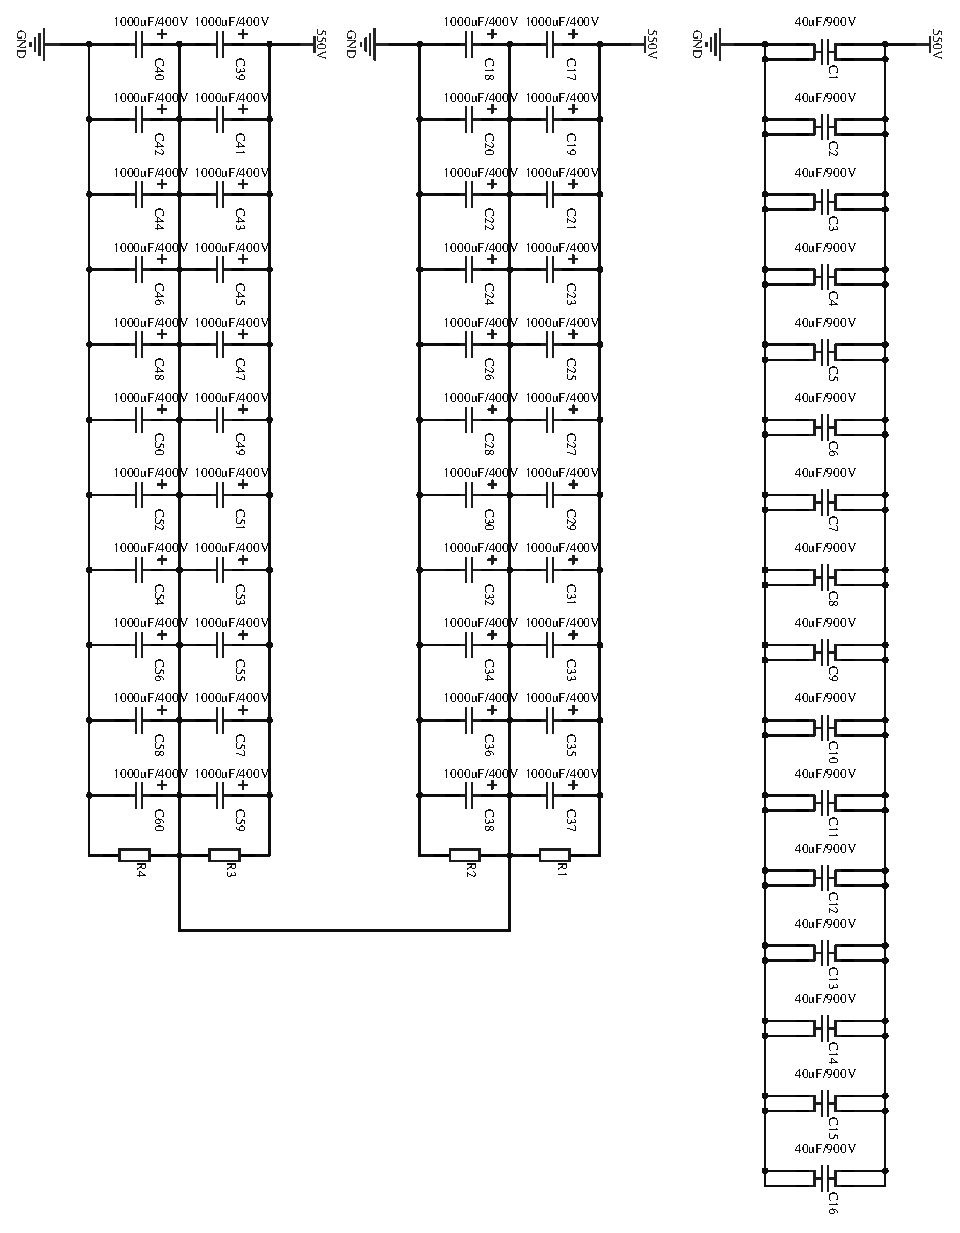
\includegraphics[width=1.1\textwidth]{schema_medziobvod_90}

\newpage
\subsection{DPS}
DPS a rozmiestnenie súčiastok (zmenšené). V poradí: top, bottom, bottom assembly:\vspace{5pt}
\centering
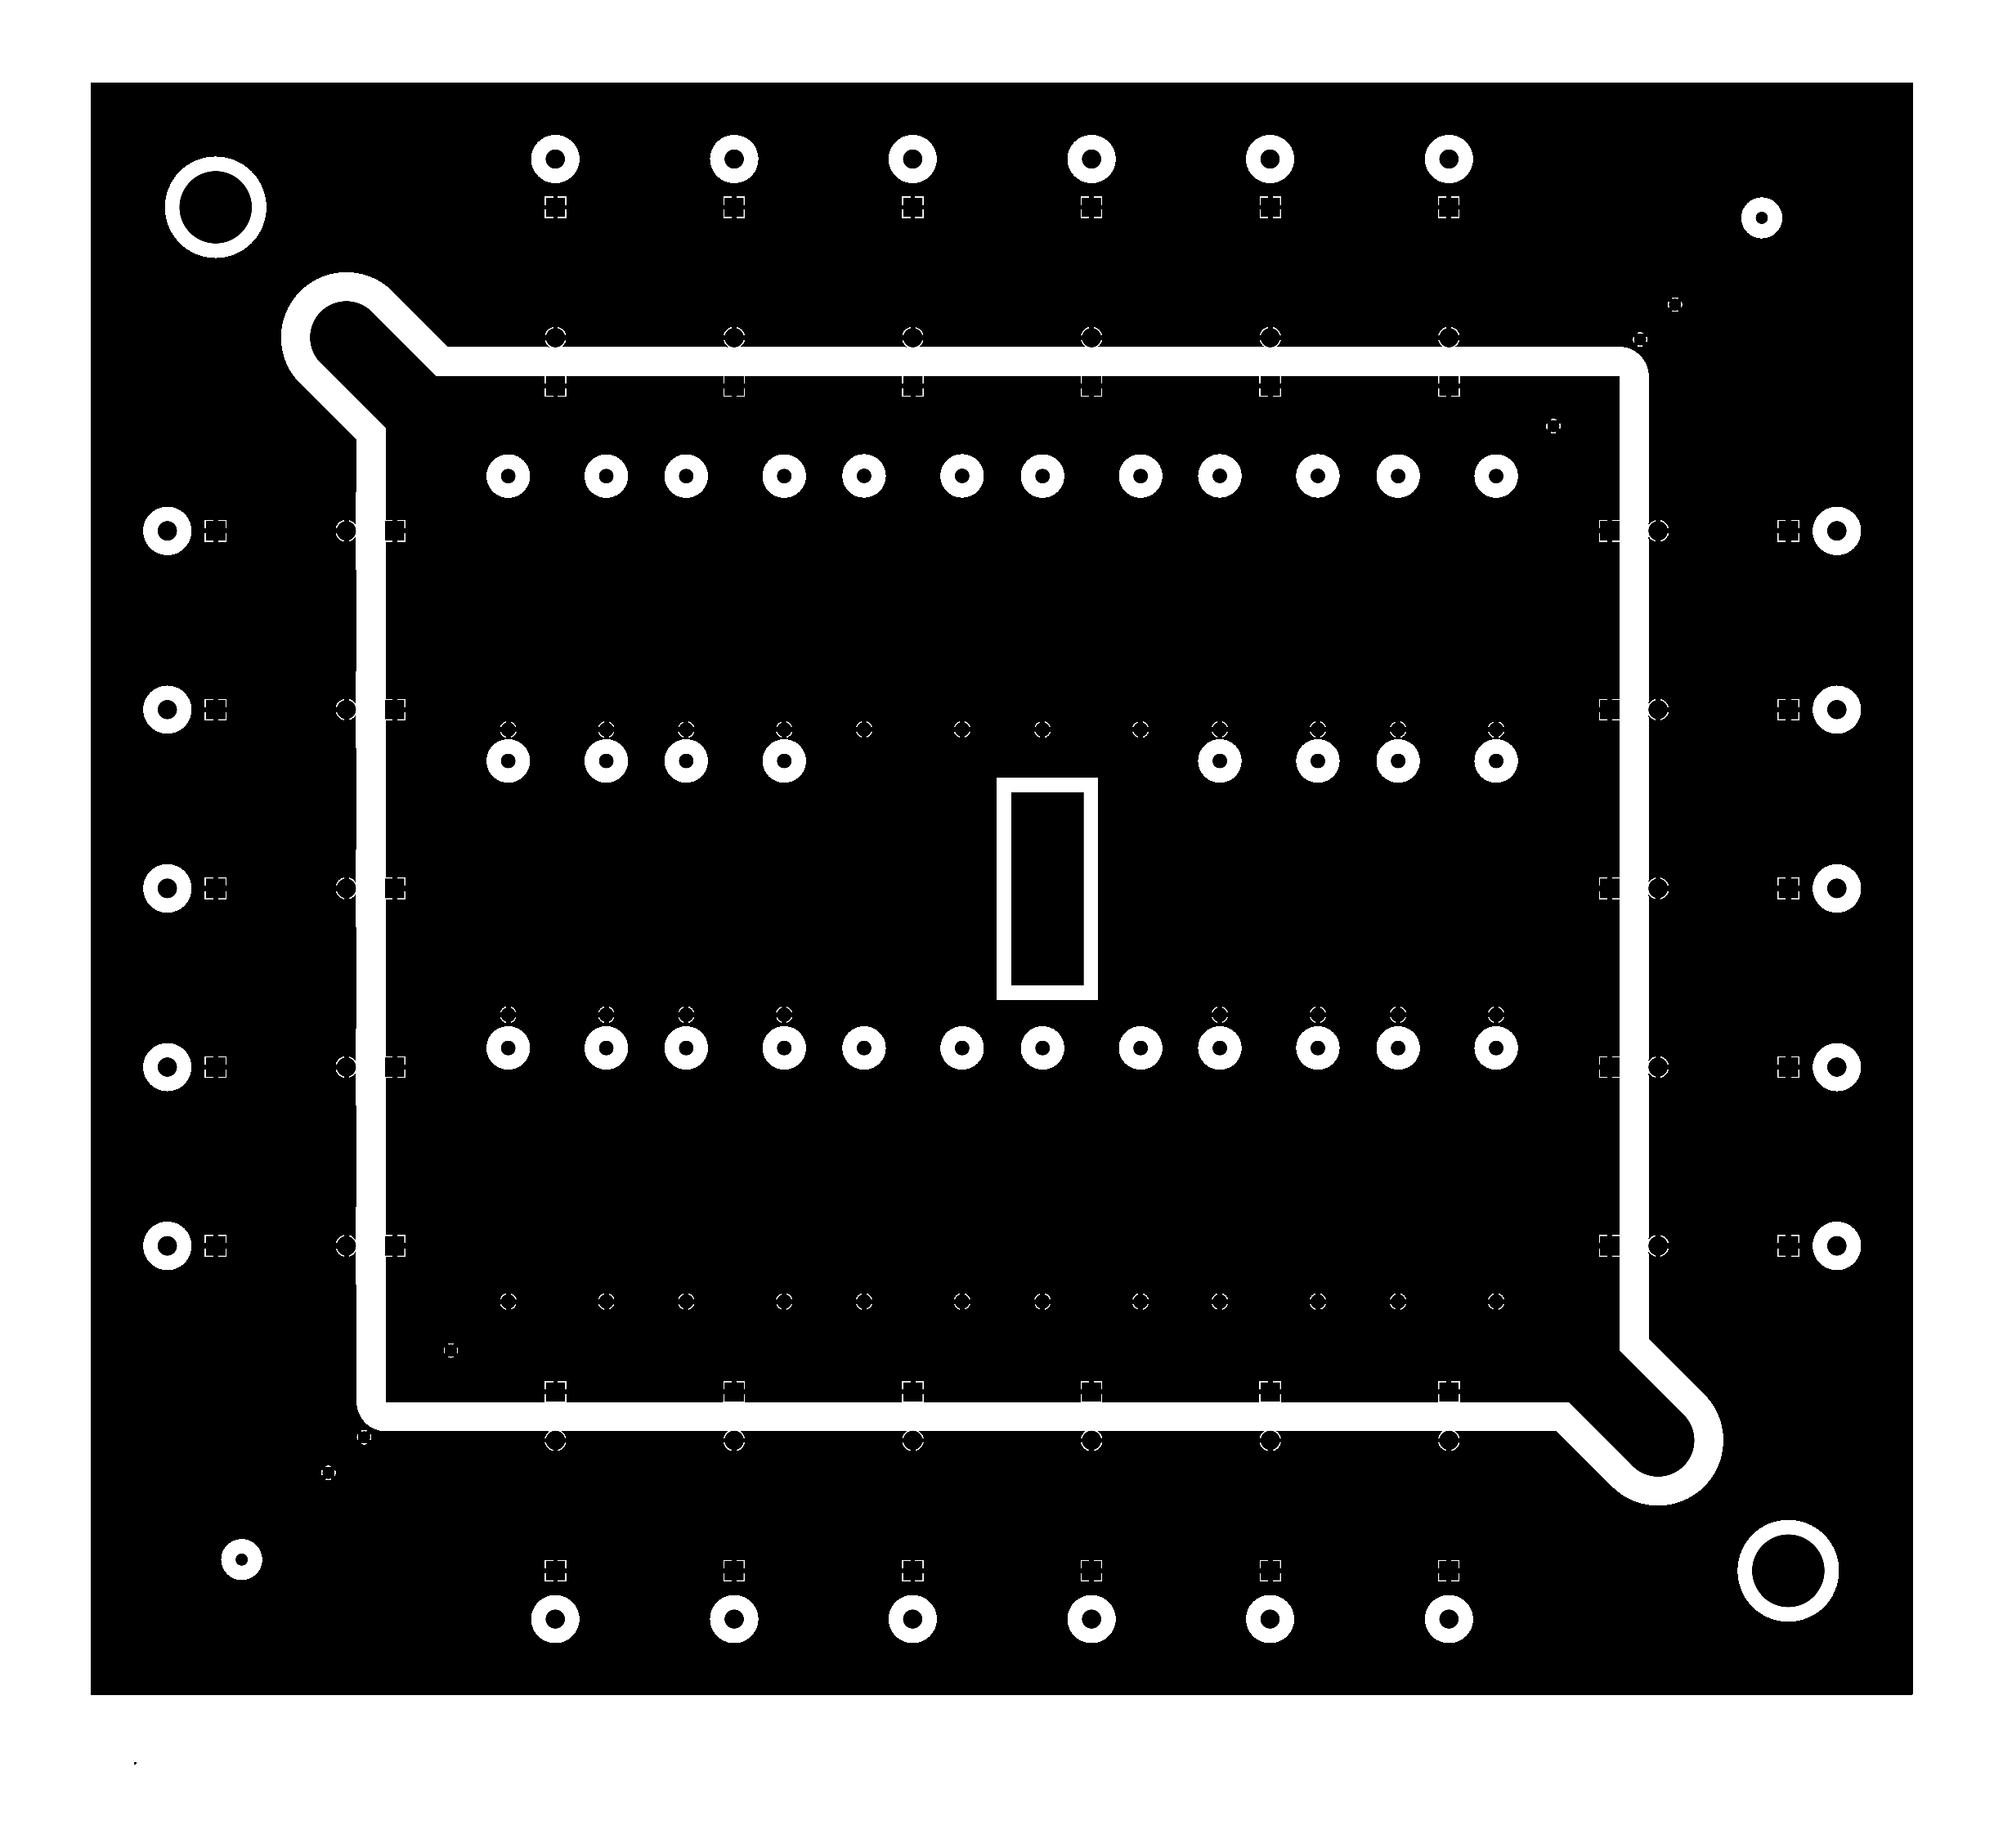
\includegraphics[width=\textwidth]{pcb_medziobvod_top}
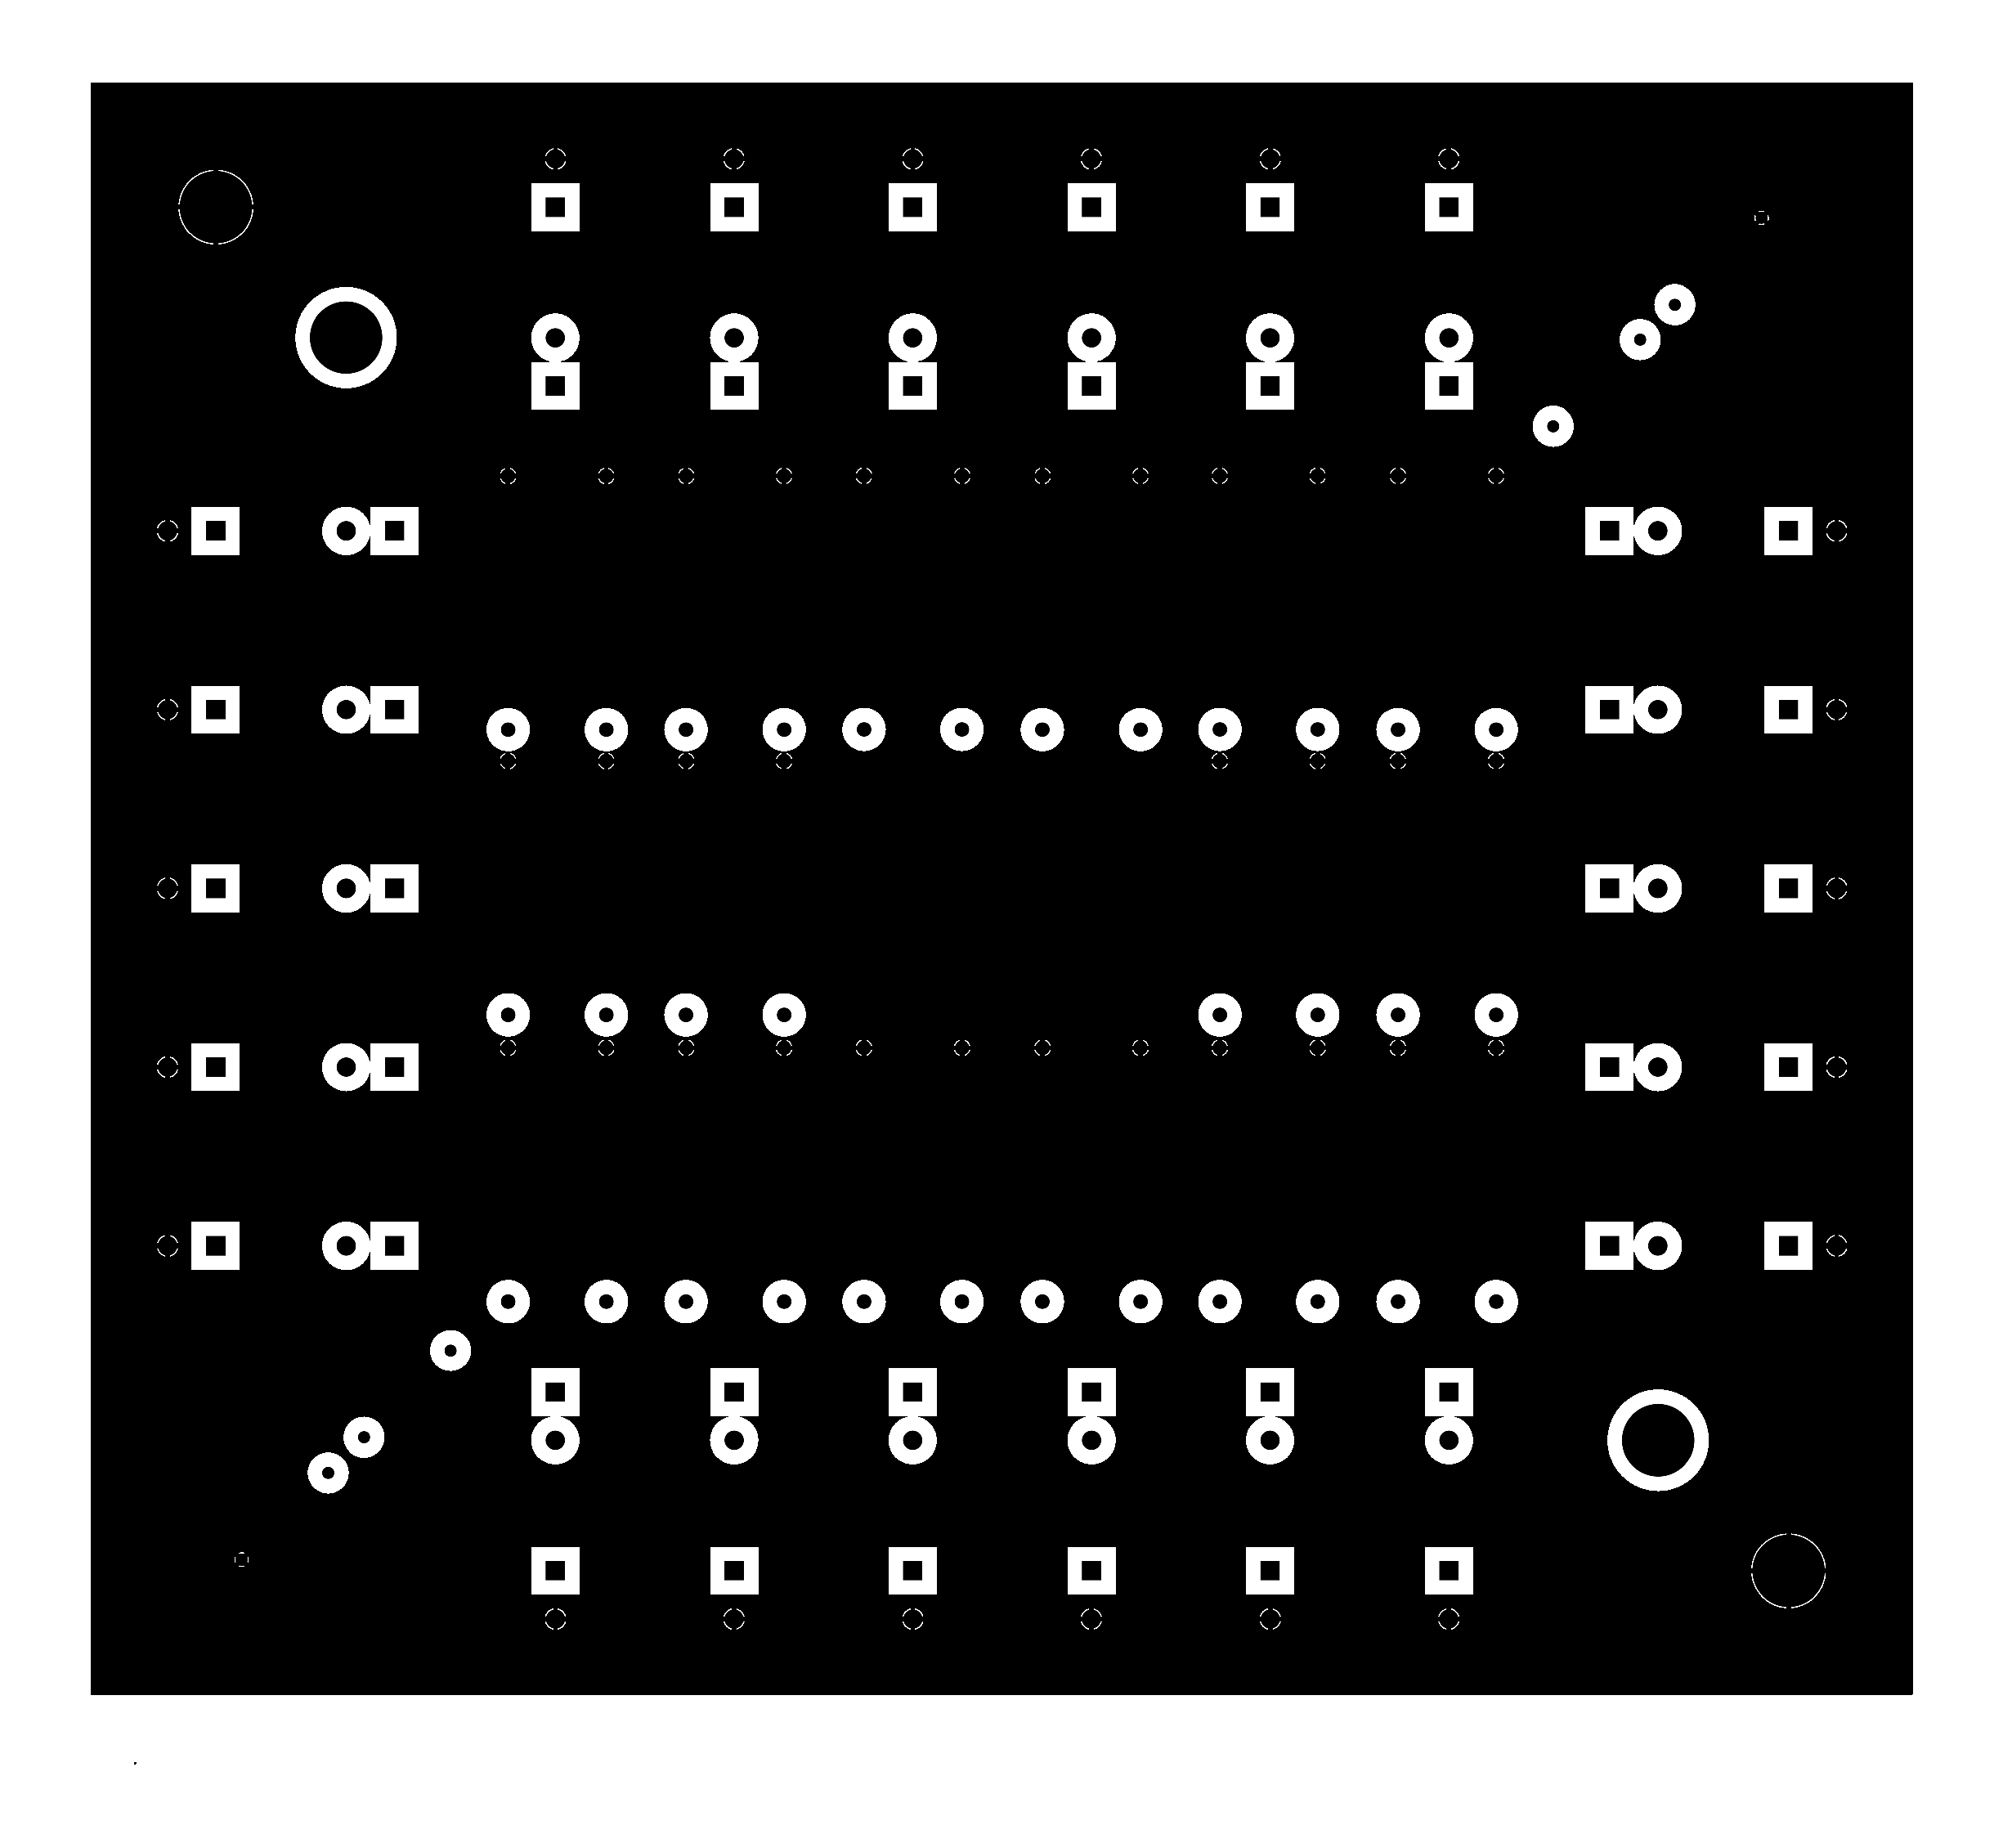
\includegraphics[width=\textwidth]{pcb_medziobvod_bot}
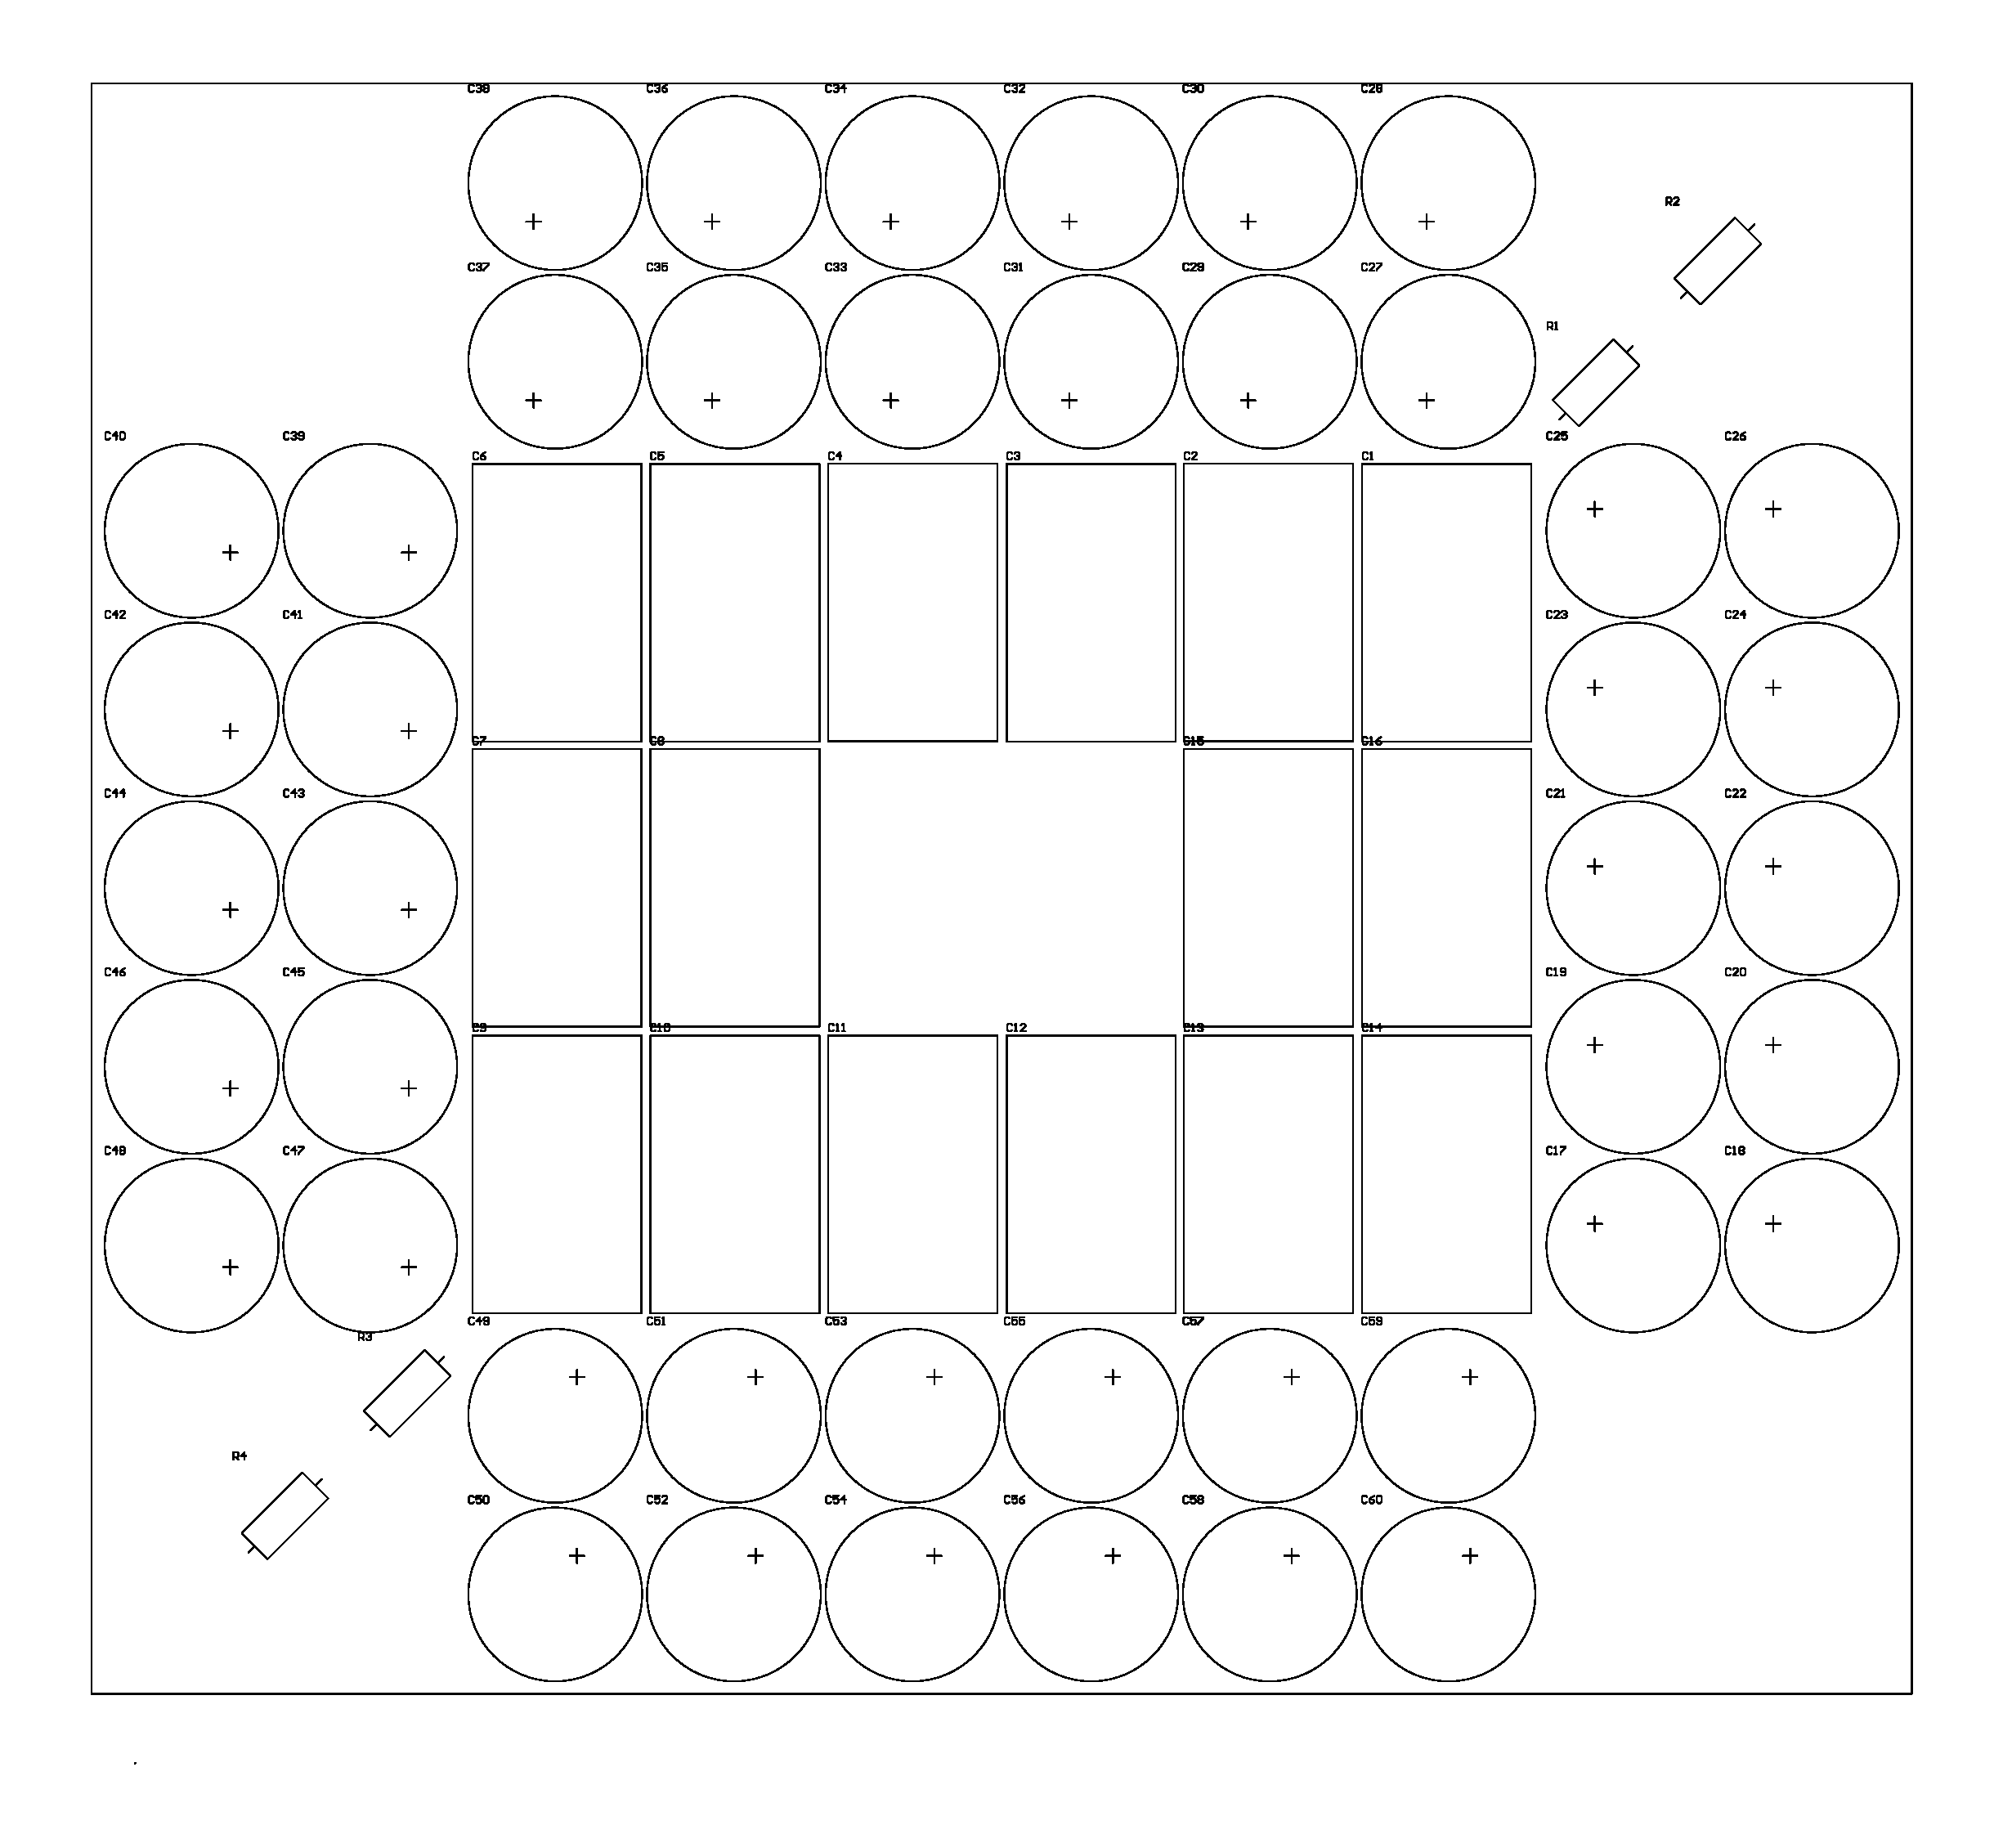
\includegraphics[width=\textwidth]{pcb_medziobvod_bot_ass}

%\newpage
%\subsection{Zoznam súčiastok}
%\small
%\hspace{2cm}
%\begin{verbatim}
%\end{verbatim}
\normalsize



\label{LastPage}
\section{Úvod}

Tady už se konečně můžete vyjádřit. Patrně bude vhodné nějaký úvod napsat,
aby se čtenář lehce vpravil do problematiky. Rozhodně ale není vhodné se
zde nějak příliš široce rozepisovat. Nezapomeňte, že pro každý příspěvek
jsou ve sborníku vyhrazeny maximálně 3 stránky pro Bc. a Mgr. studenty,
5 stran pro studenty PhD.

Když už se nám zdá, že toho bylo dost, přejdeme k věci (v další kapitole).


\section{Pokyny k psaní textu}

Pokud ke psaní textu nevyužijete šablonu, pak dodržujte následující typografické
zásady.

Velikost stránky je A4, okraje jsou 2,5~cm, pouze dolní okraj má 3,2~cm.

Hlavička se skládá z názvu příspěvku, jména autora, studijního programu, školy, 
emailu, jména školitele, emailu školitele, abstraktu a klíčových slov, a celá je
psána anglicky!

Název příspěvku: písmo Times New Roman, velikost 16~b., tučně, všechna písmena
velká, mezera za odstavcem 24~b., zarovnat na střed.

Jméno autora: písmo Times New Roman, velikost 12~b., tučně, zarovnat na střed,
mezera za odstavcem 6~b. POZOR! Jméno autora uvádějte BEZ TITULŮ!!!
                      
Studijní program, škola, a emaily: písmo Times New Roman, velikost 9~b.,
zarovnat na střed, mezera za odstavcem 6~b.Studijní program je buď 
Bachelor Degree Programme, Master Degree Programme nebo Doctoral Degree 
Programme. Číslo v závorce udává ročník, který studujete. Za čárkou následuje
ANGLICKÁ zkratka školy, kterou studujete (tedy FEEC~BUT nebo FIT~BUT).
Studenti středních škol uvedou anglický název školy a do závorky ročník,
který studují.

Jméno školitele: písmo Times New Roman, velikost 12~b., zarovnat na střed, 
mezera před odstavcem 18~b. POZOR! Jméno školitele uvádějte BEZ TITULŮ!!!

Abstrakt: písmo Times New Roman, velikost 11~b., zarovnat do bloku, odsazení 
odstavce 5~mm,  mezera před odstavcem 18~b. a za odstavcem 6~b., první slovo je 
„Abstract“ a je psáno tučně, následuje abstrakt v angličtině.

Klíčová slova: písmo Times New Roman, velikost 11~b., zarovnat do bloku, 
odsazení odstavce 5~mm, mezera za odstavcem 6~b., první slovo je „Keywords“ a je
psáno tučně, následuje seznam klíčových slov v angličtině.

Text pište fontem Times New Roman, velikost 11~b., za odstavec vkládejte 
mezeru 6~b., odsazení odstavce je 5~mm, zarovnání do bloku, řádkování jednoduché
a povolte dělení slov.

Nadpisy úrovně 1: písmo Times New Roman, velikost 11~b., tučné, všechna písmena
velká, zarovnat doleva, mezera před odstavcem 24~b., za odstavcem 6~b.

Nadpisy úrovně 2: písmo Times New Roman, velikost 11~b., tučné, kapitálky, 
zarovnat doleva, mezera před odstavcem 12~b., za odstavcem 6~b.

\subsection{Upozornění}

Není vhodné (a ani přípustné) pokoušet se o zanoření větší úrovně, než je
tato. Příspěvky, které tuto (a další podmínky) nesplní, budou autorům
vráceny k~přepracování.

\subsection{Rovnice}
%----------
% Příklad použití rovnice na samostatném řádku + odkazu z textu
%
Takto $y=ax+b$ vypadá rovnice v~textu. Důležité rovnice je ovšem vhodné
napsat na samostatný řádek:

\begin{equation} \label{rovnice}
 y = px + q
\end{equation}

V~rovnici (\ref{rovnice}) jsme ukázali, že zítra nebude pršet.

\subsection{Tabulky}
%----------
% Příklad použití tabulky
Občas se může vyskytnout potřeba prezentovat nějaká data uspořádaná
do tabulky. I~to je samozřejmě možné.

\begin{table}[h]
\begin{center}
  \begin{tabular}{|l|r|}
    \hline
    X     &   Y      \\
    \hline
    10    &  100,1   \\
    20    &  102,1   \\
    30    & $-$103,5 \\
    \hline
  \end{tabular}
  \caption{
      \rm{
      \hspace{0.1cm} Závislost veličiny X na veličině Y}}
  \label{tabulka_1}
\end{center}
\end{table}

V~tabulce \ref{tabulka_1} je uvedena závislost veličiny X na veličině Y.

\subsection{Obrázek}

No, a občas se může v~textu samozřejmě také vyskytnout
nějaký ten odkaz na obrázek. Obrázek \ref{bozka_ss.jpg} ukazuje
něco, co jste ještě neviděli.

%------------
% Příklad vložení obrázku do dokumentu.
\begin{figure}[bht]
\begin{center}
  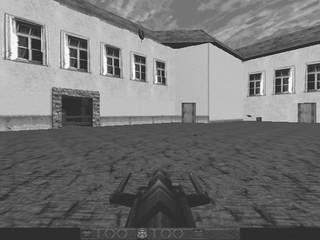
\includegraphics[width=6cm,keepaspectratio]{bozka_ss}
  \caption{
      \rm{
      \hspace{0.1cm} Obrázek Božetěchovy.}}
  \label{bozka_ss.jpg}
\end{center}
\end{figure}

\section{Závěr}
Těžko říct, co sem ještě tak asi napsat. Doufám, že tato šablonka někomu usnadní
splnění zostřených požadavků, které jsou kladeny na příspěvky pro konferenci
EEICT. Pokud bude mít někdo jakékoliv připomínky a náměty, nechť neváhá a
pošle e–mail:

\begin{center}
orsag@fit.vutbr.cz\\
drahan@fit.vutbr.cz
\end{center}

%------------
% Poděkování
%
\section*{Poděkování (anglicky = Acknowledgement)}
Tento příspěvek vznikl za podpory grantu GAČR 111/22/3333 a výzkumného
záměru XXX: J55/66:12345678 (někdo samozřejmě nemusí řešit grant nebo
něco takového, takže tuhle sekci nebudou mít ve svém příspěvku všichni.)

%------------
% Citace
%
\begin{thebibliography}{9}
  \bibitem{rybicka} Rybička, J.: \LaTeX pro začátečníky, Brno, Konvoj 1999,
            ISBN 80-85615-77-0
  \bibitem{orsag} Orság, F.: Vision für die Zukunft. Biometrie, Kreutztal,
            DE, b-Quadrat, 2004, s. 131-145, ISBN 3-933609-02-X
  \bibitem{drahansky} Drahanský, M., Orság, F.: Biometric Security Systems:
    Robustness of the Finger-print and Speech Technologies. In: BT 2004 - 
    International Workshop on Biometric Technologies, Calgary, CA, 2004,
    s. 99-103
\end{thebibliography}

\end{document}
